% !TeX program = xelatex
\documentclass[aspectratio=169,11pt]{beamer}

\usetheme{metropolis}
\metroset{block=fill,progressbar=frametitle,numbering=fraction,sectionpage=progressbar}

\usepackage{amsmath,amssymb}
\usepackage{booktabs}
\usepackage{graphicx}
\usepackage{tikz}
\usepackage{enumitem}
\usetikzlibrary{positioning}

\setlist{itemsep=2pt,topsep=2pt,parsep=0pt}

\definecolor{nanogune}{RGB}{0,96,153}
\setbeamercolor{palette primary}{bg=nanogune,fg=white}
\setbeamercolor{titlelike}{fg=nanogune}
\setbeamercolor{frametitle}{bg=nanogune,fg=white}
\setbeamercolor{progress bar}{fg=nanogune,bg=nanogune!20}
\setbeamercolor{block title}{bg=nanogune!85!black,fg=white}
\setbeamercolor{block body}{bg=nanogune!8}
\setbeamerfont{block title}{size=\small}
\setbeamerfont{block body}{size=\small}

\graphicspath{{figs/}}

\title{Magnetic Coupling in Nanographenes}
\subtitle{Visual summary --- 7-AGNR end states \& the triangulene--phenalenyl spin chain}
\author{L.~Zulueta}
\institute{CIC nanoGUNE, Donostia--San Sebasti\'an, Spain}
\date{\today}

\begin{document}

\maketitle

% =========================================================
\section{7-AGNR}
% =========================================================

\begin{frame}{Motivation: topological end states in finite 7-AGNRs}
  \begin{itemize}
    \item 7-AGNRs belong to the $N=3p+1$ family ($p=2$): semiconducting, synthesized by on-surface polymerization/cyclodehydrogenation of DBBA precursors on Au(111).
    \item Finite-length ribbons host \alert{spin-polarized topological end states} (SPTEs) at their zigzag-terminated ends, each carrying $S \approx 1/2$.
    \item Origin: a nontrivial $\mathbb{Z}_2$ (Zak-phase) invariant of the bulk bands $\Rightarrow$ bulk--boundary correspondence guarantees in-gap boundary modes, independent of edge details.
    \item \textbf{Key question:} what is the exchange coupling $J(L)$ between the two end spins, and how does it scale with ribbon length $L$ (number of DBBA monomers)?
  \end{itemize}
\end{frame}

\begin{frame}{Theoretical framework: Hamiltonian}
  \textbf{Third-nearest-neighbour tight-binding} on the $p_z$ lattice:
  \[
    H_{\mathrm{TB}} = -\sum_{\langle i,j\rangle} t_1\, c_i^\dagger c_j - \sum_{\langle\langle i,j\rangle\rangle} t_2\, c_i^\dagger c_j - \sum_{\langle\langle\langle i,j\rangle\rangle\rangle} t_3\, c_i^\dagger c_j + \mathrm{H.c.}
  \]
  \begin{center}
  \begin{tabular}{cccc}
    \toprule
    $t_1$ & $t_2$ & $t_3$ & $U$ (Hubbard) \\
    \midrule
    $-2.7$~eV & $-0.2$~eV & $-0.18$~eV & $3.0$~eV \\
    \bottomrule
  \end{tabular}
  \end{center}
  \textbf{Mean-Field Hubbard (MFH):} $H = H_{\mathrm{TB}} + U\sum_i n_{i\uparrow} n_{i\downarrow}$, decoupled self-consistently (SCF tolerance $10^{-13}$ on the density matrix).
  \[
    m_i = \langle n_{i\uparrow}\rangle-\langle n_{i\downarrow}\rangle \quad\text{(local magnetic moment)}
  \]
\end{frame}

\begin{frame}{Two independent routes to the exchange coupling $J$}
  \begin{block}{1. Self-consistent MFH total energies}
    \[
      J = E_{\mathrm{FM}} - E_{\mathrm{AFM}}
    \]
    AFM: open-shell singlet, $S_z=0$. FM: triplet enforced via $q=(N/2{+}1, N/2{-}1)$, $S_z=1$.
  \end{block}
  \begin{block}{2. Effective Hubbard dimer (Anderson superexchange)}
    \[
      t_{\mathrm{eff}} = \tfrac{1}{2}|\varepsilon_{\mathrm{LUMO}}-\varepsilon_{\mathrm{HOMO}}|, \qquad
      U_{\mathrm{eff}} = U\sum_i |\psi_L(i)|^4, \qquad
      J = \frac{4\,t_{\mathrm{eff}}^2}{U_{\mathrm{eff}}}
    \]
    $\psi_L = (\psi_{\mathrm{HOMO}}+\psi_{\mathrm{LUMO}})/\sqrt{2}$: reconstructed localized end-state orbital.
  \end{block}
  Since $t_{\mathrm{eff}}\propto e^{-L/\xi_0}$: $J(L)=Ae^{-L/\xi}$ is predicted to decay exponentially.
\end{frame}

\begin{frame}{Geometry check}
  \centering
  
\includegraphics[width=0.97\textwidth]{test_geom_L4.png}
  \begin{itemize}
    \item Pruned, zigzag-terminated 7-AGNR, $L=4$ DBBA monomers.
  \end{itemize}
\end{frame}

\begin{frame}{Spin-polarized end states ($L=6$)}
  \centering
  
\includegraphics[width=0.78\textwidth]{spin_polarization_L6.png}
  \begin{itemize}
    \item AFM (top, $S_z{=}0$) vs.\ FM (bottom, $S_z{=}1$) --- moments localized at the two ends.
  \end{itemize}
\end{frame}

\begin{frame}{Dimer vs.\ Heisenberg (MFH)}
  \centering
  
\includegraphics[width=0.74\textwidth]{J_comparison_vs_L.png}
  \begin{itemize}
    \item Both routes agree: $J(L)=Ae^{-L/\xi}$, $\xi = 0.38$ DBBA monomers.
  \end{itemize}
\end{frame}

% =========================================================
\section{Triangulene--Phenalenyl Copolymer}
% =========================================================

\begin{frame}{Motivation: chemically designed spin chains}
  \begin{itemize}
    \item Complementary strategy to ribbon end states: assemble a spin chain from \alert{chemically localized radical building blocks}.
    \item Repeating motif $P\text{--}T\text{--}P$ under open boundary conditions: $P\text{--}T\text{--}P\text{--}[P\text{--}T\text{--}P]_{N-1}$.
    \item \textbf{Phenalenyl (P):} alternant radical, sublattice imbalance $1$ $\Rightarrow$ single $S=\tfrac12$ moment.
    \item \textbf{[3]Triangulene (T):} sublattice imbalance $2$ $\Rightarrow$ $S=1$ moment; represented as two $S=\tfrac12$ sites $T_a,T_b$ locked into a triplet by a strong \emph{ferromagnetic} intra-unit exchange $J_T<0$.
    \item Every monomer maps onto four $S=\tfrac12$ nodes $[\,P,T_a,T_b,P\,]$; the oligomer maps onto a chain of $n=4N$ spin-$\tfrac12$ sites.
  \end{itemize}
\end{frame}

\begin{frame}{Copolymer geometry}
  \centering
  
\includegraphics[width=0.60\textwidth]{oligomer_closed.png}
  \begin{itemize}
    \item $P$--$T$--$P$ oligomer, $N=1$, closed-shell reference structure.
  \end{itemize}
\end{frame}

\begin{frame}{MFH ground-state spin density: single monomer ($N=1$)}
  \centering
  
\includegraphics[width=0.55\textwidth]{spin_density_monomer1.png}
  \begin{itemize}
    \item Open-shell singlet ground state, $S_z=0$ (MFH, $U=3.0$~eV): total $\sum_i|m_i| = 6.50$.
    \item Spin density directly visualizes the $P$ ($S{=}1/2$) and $T$ ($S{=}1$, on $T_a,T_b$) building blocks predicted by sublattice-imbalance counting.
  \end{itemize}
\end{frame}

\begin{frame}{MFH spin density (trimer, $N=3$)}
  \centering
  
\includegraphics[width=0.92\textwidth]{spin_density_monomer3.png}
  \begin{itemize}
    \item Open-shell singlet, $S_z=0$; alternating $P$/$T$ moments along the chain.
  \end{itemize}
\end{frame}

\begin{frame}{From MFH to an effective Heisenberg spin chain}
  \[
    H = \sum_{m=0}^{N-1}\Big[J_{TP}\big(\mathbf S_{4m}\!\cdot\!\mathbf S_{4m+1} + \mathbf S_{4m+2}\!\cdot\!\mathbf S_{4m+3}\big) + J_T\, \mathbf S_{4m+1}\!\cdot\!\mathbf S_{4m+2}\Big] + J_{PP}\!\!\sum_{m=0}^{N-2}\!\! \mathbf S_{4m+3}\!\cdot\!\mathbf S_{4m+4}
  \]
  \centering
  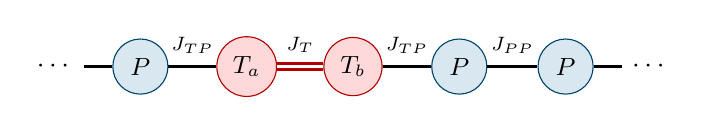
\begin{tikzpicture}[
      P/.style={circle,draw=nanogune!70!black,fill=nanogune!15,minimum size=7mm,font=\small},
      T/.style={circle,draw=red!70!black,fill=red!15,minimum size=7mm,font=\small},
      afm/.style={thick},
      fm/.style={very thick,red!70!black,double,double distance=1pt},
      lbl/.style={font=\scriptsize,midway,above=1pt},
      x=1.35cm]
    \node (l0) at (-0.8,0) {$\cdots$};
    \node[P] (P1) at (0,0) {$P$};
    \node[T] (Ta) at (1,0) {$T_a$};
    \node[T] (Tb) at (2,0) {$T_b$};
    \node[P] (P2) at (3,0) {$P$};
    \node[P] (P3) at (4,0) {$P$};
    \node (r0) at (4.8,0) {$\cdots$};
    \draw[afm] (l0)--(P1);
    \draw[afm] (P1)--(Ta) node[lbl]{$J_{TP}$};
    \draw[fm]  (Ta)--(Tb) node[lbl,black]{$J_{T}$};
    \draw[afm] (Tb)--(P2) node[lbl]{$J_{TP}$};
    \draw[afm] (P2)--(P3) node[lbl]{$J_{PP}$};
    \draw[afm] (P3)--(r0);
  \end{tikzpicture}
  \vspace{1mm}
  \begin{center}
  \begin{tabular}{ccc}
    \toprule
    $J_{PP}$ (AFM) & $J_{TP}$ (AFM) & $J_T$ (FM) \\
    \midrule
    $38$~meV & $40$~meV & $-500$~meV \\
    \bottomrule
  \end{tabular}
  \end{center}
  Since $|J_T|\gg J_{TP},J_{PP}$: each $(T_a,T_b)$ pair freezes into an effective $S=1$ object $\Rightarrow$ mixed $\tfrac12$--$1$--$\tfrac12$ AFM spin chain.
\end{frame}

\begin{frame}{Exact-diagonalization spin texture}
  \centering
  
\includegraphics[width=0.95\textwidth]{spin_chain_N3_crop.png}
  \begin{itemize}
    \item Singlet ground state; lowest triplet shown --- singlet--triplet gap $\Delta = 11.04$~meV.
  \end{itemize}
\end{frame}

\begin{frame}[standout]
  To be continued\\
  \vspace{6mm}
  \begin{tikzpicture}
    \draw[white, line width=3pt] (0,0) circle (1.3);
    \fill[white] (-0.5,0.4) circle (0.14);
    \fill[white] (0.5,0.4) circle (0.14);
    \draw[white, line width=3pt] (-0.6,-0.25) arc (200:340:0.65);
  \end{tikzpicture}
\end{frame}

\end{document}
